\section{Evaluation}
\label{sec:eval}
\begin{figure}[t]
{
\setlength{\belowcaptionskip}{-15pt}
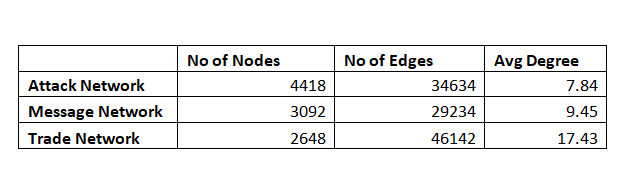
\includegraphics[width=\linewidth]{pics/1542805929316blob.jpg}  
\caption{Statistics on our Travian dataset}
\label{fig:algo2} 
}
\end{figure}

\input{dataset-graphs}

\input{result-table}
\input{dataset-jeffi}

\subsection{Dataset}
\label{sec:dataset}

The Travian dataset contains three networks which are Trade, Message and
Attack. The data is  present in graphml and csv formats. The three graphs are
unweighted and undirected and contains three fields for each of the networks
they are timestamp of the event be it message, trade or attack, node1 and
node2. For all the three networks we have calculated the total number of
distinct nodes, the toal number of distinct edges and the average dergree per
node for all the 30 snapshots.The data for this has been summarised in the
table~\ref{tab:data}. We can see that the trade graph is more connected than
the  other two graphs although the total number of nodes trading is lesser
than the ones  messaging or attacking.



% For the graphs 2, 3 and 4 they represent the cases for dynamic multiplex link prediction using the Jaccard Coefficient similarity measure.






% Talk about the source of dataset and its characteristics.

% \subsubsection{Characteristics}

% We need to collect some statistics on our dataset.

% \subsubsection{Optimization}

% Describe what changes did we have to do to our dataset.


\subsection{Results}

As mentioned in section~\ref{sec:implementation}, we perform dyamic single
layer link prediction,  multiplex link prediction using Algorithm
1~\ref{fig:algo1} and Algorithm 2~\ref{fig:algo2} on our dataset. For all the
cases, we take the snapshots of first $21$ days as  our train dataset and
predict the links for last $9$ days. We use AUROC score to gauge our
predictions, for each day we calculate the AUROC score and report the average
score for the last $9$ days. Our results are summarized in table~\ref{tab:res}. 

For the dyamic single layer link prediction case, we get a maximum score of
$0.3575$ using  Preferential Attachment and it does not vary a lot for the other
metrics. In the case of multiplex link prediction, we calculate the scores for
trade on attack, message on attack and for both trade and message on attack.
In the naive case, Clustering coefficient  metric gives the best results
$0.4307$ when used for multiplex link prediction for the trade and message on
attack case while Shortest Path gives the worst with an average AUROC score of
$0.2472$. We perform Borda's rank aggregation for all the metrics in naive
case and we get $0.4914$ for the combined(trade + message) case. Finally, the
AUROC score using Algorithm1 is $0.5542$ for the combined case and  $0.5763$
for Algorithm2. 
 
We also give some visualizations for both single and multiplex layer link
prediction. We use Jaccards Coefficient for this purpose. Graph~\ref{fig:jf1}
showcases the top $1000$ links predicted on the attack layer when the
prediction was made by studying the effect of attack layer on itself.
Graph~\ref{fig:jf2} showcases the top $1000$ links predicted on the attack
layer when the prediction was made by studying the effect of trade layer on
the attack layer.  Graph~\ref{fig:jf3} showcases the top $1000$ links
predicted on the attack layer when the prediction was made by studying the
effect of message layer on the attack layer.  Graph~\ref{fig:jf4} showcases
the top $1000$ links predicted on the attack layer when the prediction was
made by studying the combined effect of message and trade layers on the attack
layers.

\subsection{Analysis}

For the naive case in multiplex link prediction, we can infer from the table
that most metrics(except Shortest Path) give  better results than the single
layer link prediction. The highest difference can be observed with Clustering
Coefficient  which outputs an AUROC score of $0.4307$ for the combined case in
comparison to $0.3540$ for prediction using just the attack layer. However, we
can  see that the naive case does not perform as good as the algorithm 1 which
leverages  cross layer features by using the Likelyhood Assigment and Edge
weighting functions. In fact,  the algorithm1 also outperforms Borda Rank
aggregation over the similarity metrics in the naive case.

Our proposed algorithm performs even better than algorithm1 in all the cases
thus,  giving the highest accuracy amongst all methods. As mentioned, this is
because it  incorporates more network features when compared to other methods.











